% Included from both -slides and -handout versions.

\mode<presentation>
{
  \usetheme{default}
  \useoutertheme{infolines}
}

\usepackage[english]{babel}
\usepackage[latin1]{inputenc}
\usepackage{graphicx}
\usepackage{times}
\usepackage[T1]{fontenc}
\usepackage{fancyvrb}
\usepackage{listings}
\begin{document}
\lstset{language=C, escapeinside={(*@}{@*)}, numbers=left,
  basicstyle=\tiny, showspaces=false, showtabs=false}

\def\Tiny{\fontsize{4pt}{4pt} \selectfont}

\title{L41 - Lecture 5: The Network Stack (1)}
%\institute{University of Cambridge}
%\author{George V. Neville-Neil}
\author{Dr Robert N. M. Watson}
\date{19 January 2016}

\begin{frame}
  \titlepage
\end{frame}

\section{Introduction}

\begin{frame}
  \frametitle{Reminder: where we left off in Michaelmas Term}

  \pause

  Long, long ago, but in a galaxy not so far away:

  \begin{itemize}
    \item Lecture 3: The Process Model (1)
    \item Lecture 4: The Process Model (2)

    \pause
    \medskip

    \item Lab 1: I/O performance

    \pause
    \medskip

    \item Lab 2: IPC buffer size and probe effect
    \item Lab 3: Micro-architectural effects of IPC
  \end{itemize}

  \pause
  \medskip

  Explored several implied (and rejected) hypotheses:

  \begin{itemize}
    \item Larger I/O and IPC buffer sizes amortize system-call overheads

    \pause

    \item Micro-architecture is irrelevant

    \pause

    \item The probe effect doesn't matter in real workloads
  \end{itemize}
\end{frame}

\begin{frame}
  \frametitle{This time: Introduction to the Network Stack}

  Rapid tour across hardware and software:

  \medskip

  \begin{enumerate}
    \item Networking and the sockets API
    \item Network-stack design principles: 1980s and today
    \item Memory flow across hardware and software
    \item Network-stack construction and work flows
    \item Recent network-stack research
  \end{enumerate}
\end{frame}

\section{Network-stack goals}

\begin{frame}
  \frametitle{Networking: a key OS function}

  \pause
  \medskip

  \begin{itemize}
    \item Communication between distributed computer systems
    \begin{itemize}
      \item \textit{Local-area networking} (LANs) and
	\textit{wide-area networking} (WANs)
    \end{itemize}

    \pause
    \medskip

    \item A network stack provides:
    \begin{itemize}
      \item Sockets API and extensions
      \item Interoperable, feature-rich, high-performance protocol
	implementations (e.g., IPv4, IPv6, ICMP, UDP, TCP, SCTP, ...)
      \item Device drivers for Network Interface Cards (NICs)
      \item Monitoring and management interfaces (BPF, \texttt{ioctl})
      \item Plethora of support libraries (e.g., DNS)
    \end{itemize}

    \pause
    \medskip

    \item Dramatic changes over 30 years:
    \begin{itemize}
      \item 1980s: Early packet-switched networks, UDP+TCP/IP, Ethernet
      \item 1990s: Large-scale migration to IP; Ethernet VLANs
      \item 2000s: 1-Gigabit/s, then 10-Gigabit/s Ethernet; 802.11, GSM data
      \item 2010s: Large-scale deployment of IPv6; 40/100-Gigabit/s Ethernet
    \end{itemize}

    \medskip
    \pause

    \item Vanishing technologies: UUCP, IPX/SPX, ATM, token ring, SLIP, ...
  \end{itemize}
\end{frame}

\begin{frame}
  \frametitle{The Berkeley Sockets API (1983)}

  \begin{columns}[T]
    \column{0.125\textwidth}
      \bigskip
      \begin{scriptsize}
	\texttt{close()} \\
	\texttt{read()} \\
	\texttt{write()} \\
	...

	\bigskip

	\texttt{accept()} \\
	\texttt{bind()} \\
	\texttt{connect()} \\
	\texttt{getsockopt()} \\
	\texttt{listen()} \\
	\texttt{recv()} \\
	\texttt{select()} \\
	\texttt{send()} \\
	\texttt{setsockopt()} \\
	\texttt{socket()} \\
	...
      \end{scriptsize}

    \pause

    \column{0.775\textwidth}
    \begin{itemize}
      \item \textit{The Design and Implementation of the 4.3BSD Operating
	System} (although appeared in 4.2)
      \item Now universal TCP/IP API (POSIX, Windows, ...)

      \pause
      \medskip

      \item Kernel-resident network stack serves userspace networking
	applications via system calls
      \item Reuse file-descriptor abstraction
      \begin{itemize}
	\item Same API for local and distributed IPC
	\item Simple, synchronous, copying semantics
	\item Blocking/non-blocking I/O, \texttt{select()}
      \end{itemize}

      \pause
      \medskip

      \item Multi-protocol (e.g., IPv4, IPv6, ISO, ...)
      \begin{itemize}
	\item TCP-focused but not TCP-specific
	\item Cross-protocol abstractions and libraries
	\item Protocol-specific implementations
	\item ``Portable'' applications
      \end{itemize}

      %\pause
      %\medskip
      %
      %\item NB: `socket' in BSD API != `socket' in TCP RFC
    \end{itemize}
  \end{columns}
\end{frame}

\begin{frame}
  \frametitle{BSD network-stack principles (1980s-1990s)}

   A framework for \textbf{multi-protocol}, \textbf{packet-oriented} network
   research:

   \medskip
   \pause

  \begin{itemize}
    \item Object-oriented: multiple protocols, multiple socket types, one API
    \begin{itemize}

      \pause

      \item \textbf{Protocol-independent}: streams vs. datagrams, sockets,
	socket buffers, socket addresses, network interfaces, routing table,
	packets

      \pause

      \item \textbf{Protocol-specific}: connection lists, address/routing
	specialization, routing, transport protocol itself -- encapsulation,
	decapsulation, etc
    \end{itemize}

    \medskip
    \pause

    \item Fundamentally packet-oriented design:
    \begin{itemize}
      \item Packets and packet queueing as fundamental primitives

      \pause

      \item If there is a failure (overload, corruption) drop the packet

      \pause

      \item Work hard to maintain packet source ordering

      \pause

      \item Differentiate `receive' from `deliver' and `send' from `transmit'

      \pause

      \item Heavy focus on TCP functionality and performance

      \pause

      \item Middle-node (forwarding), not just edge-node (I/O), functionality 

      \pause

      \item High-performance packet capture: Berkeley Packet Filter (BPF)
    \end{itemize}
%    \item In-kernel consumers, such as NFS, supported using sockets KPI
  \end{itemize}
\end{frame}

\begin{frame}
  \frametitle{FreeBSD network-stack principles (1990s-2010s)}

  All of the 1980s features and also ...

  \medskip
  \pause

  \begin{itemize}
    \item Hardware:
    \begin{itemize}
      \item Multi-processor scalability
      \item NIC offload features (checksums, TSO/LRO, full TCP)
      \item Multi-queue network cards with load balancing/flow direction
      \item Performance to 10s or 100s of Gigabit/s
      \item Wireless networking
    \end{itemize}

    \medskip
    \pause

    \item Protocols:
    \begin{itemize}
      \item Dual-IPv4/IPv6
      \item Security/privacy: firewalls, IPsec, ...
    \end{itemize}

    \medskip
    \pause

    \item Software model:
    \begin{itemize}
      \item Flexible memory model integrates with VM for zero-copy
      \item Network-stack virtualisation
      \item Userspace networking via \texttt{netmap}
    \end{itemize}
  \end{itemize}
\end{frame}

\section{Network-stack design}

\begin{frame}
  \frametitle{Memory flow in hardware}

  \begin{center}
  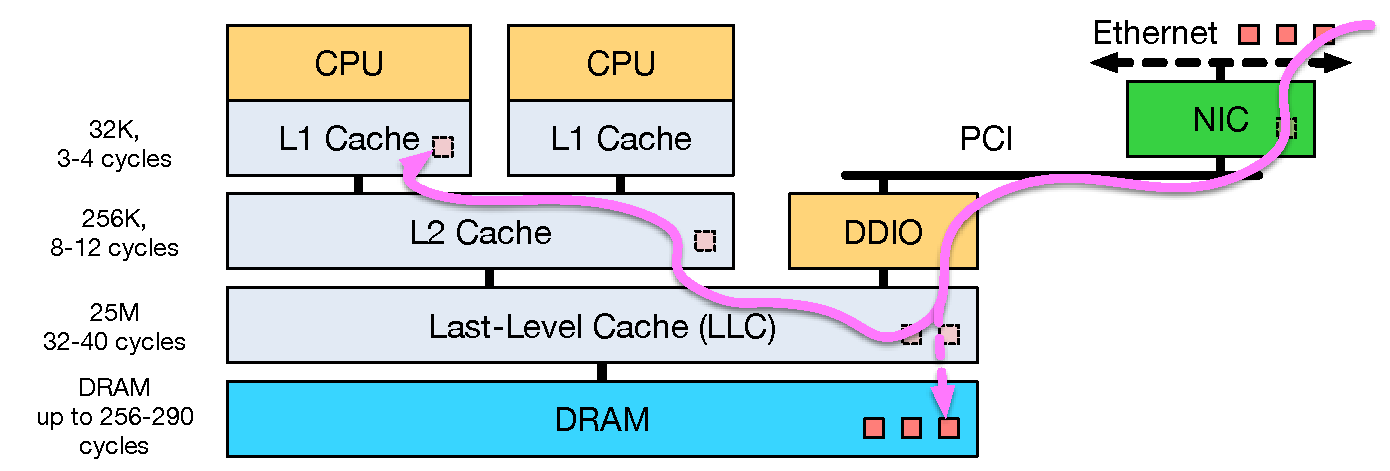
\includegraphics[scale=0.5]{../../figures/network-cpu-ddio-nic.pdf}
  \end{center}

  \medskip
  \pause

  \begin{itemize}
    \item Key idea: \textit{follow the memory}

    \medskip
    \pause

    \item Historically, memory copying avoided due to CPU cost
    \item Today, memory copying avoided due to cache footprint

    \medskip
    \pause

    \item Recent Intel CPUs push and pull DMA via the LLC (``DDIO'')
    \item NB: if we differentiate `send' and `transmit', is this a good idea?
  \end{itemize}
\end{frame}

\begin{frame}
  \frametitle{Memory flow in software}

  \begin{center}
    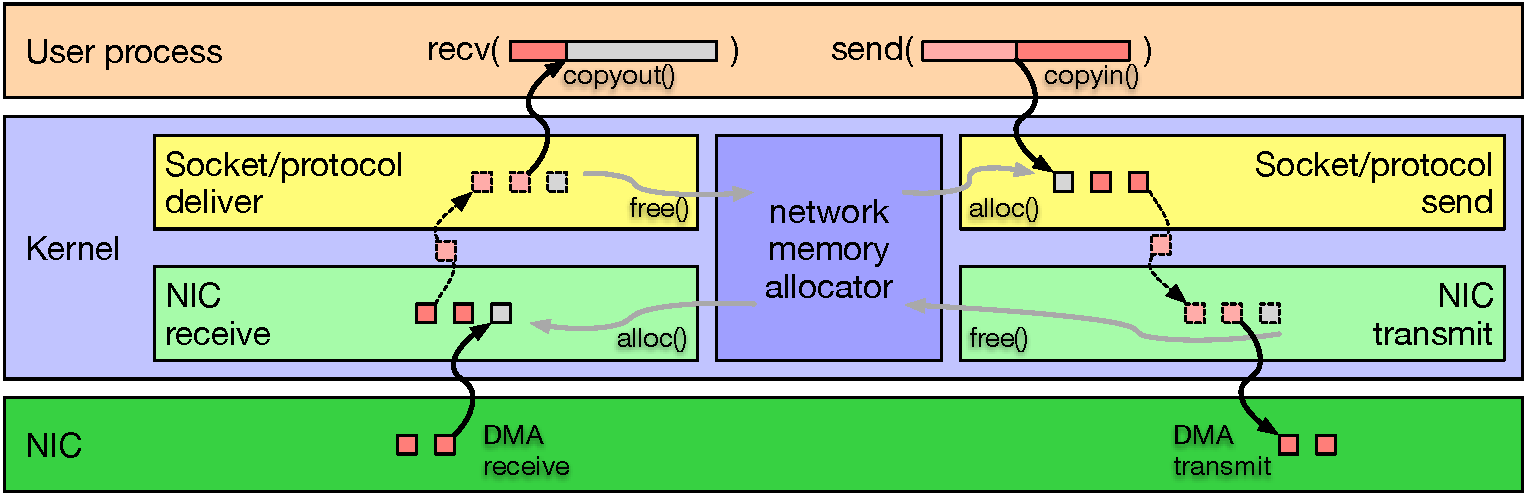
\includegraphics[width=\textwidth]{../../figures/network-memory-flow.pdf}
  \end{center}

  \pause

  \begin{itemize}
    \item Socket API implies one copy to/from user memory
    \begin{itemize}
      \item Historically, zero-copy VM tricks for socket API ineffective
    \end{itemize}

    \medskip
    \pause

    \item Network buffers cycle through the slab allocator
    \begin{itemize}
      \item Receive: allocate in NIC driver, free in socket layer
      \item Transmit: allocate in socket layer, free in NIC driver
    \end{itemize}

    \medskip
    \pause

    \item DMA performs second copy; can affect cache/memory bandwidth
    \begin{itemize}
      \item NB: what if packet-buffer working set is larger than the cache?
    \end{itemize}
  \end{itemize}
\end{frame}

\begin{frame}
  \frametitle{The \texttt{mbuf} abstraction}

  \begin{center}
    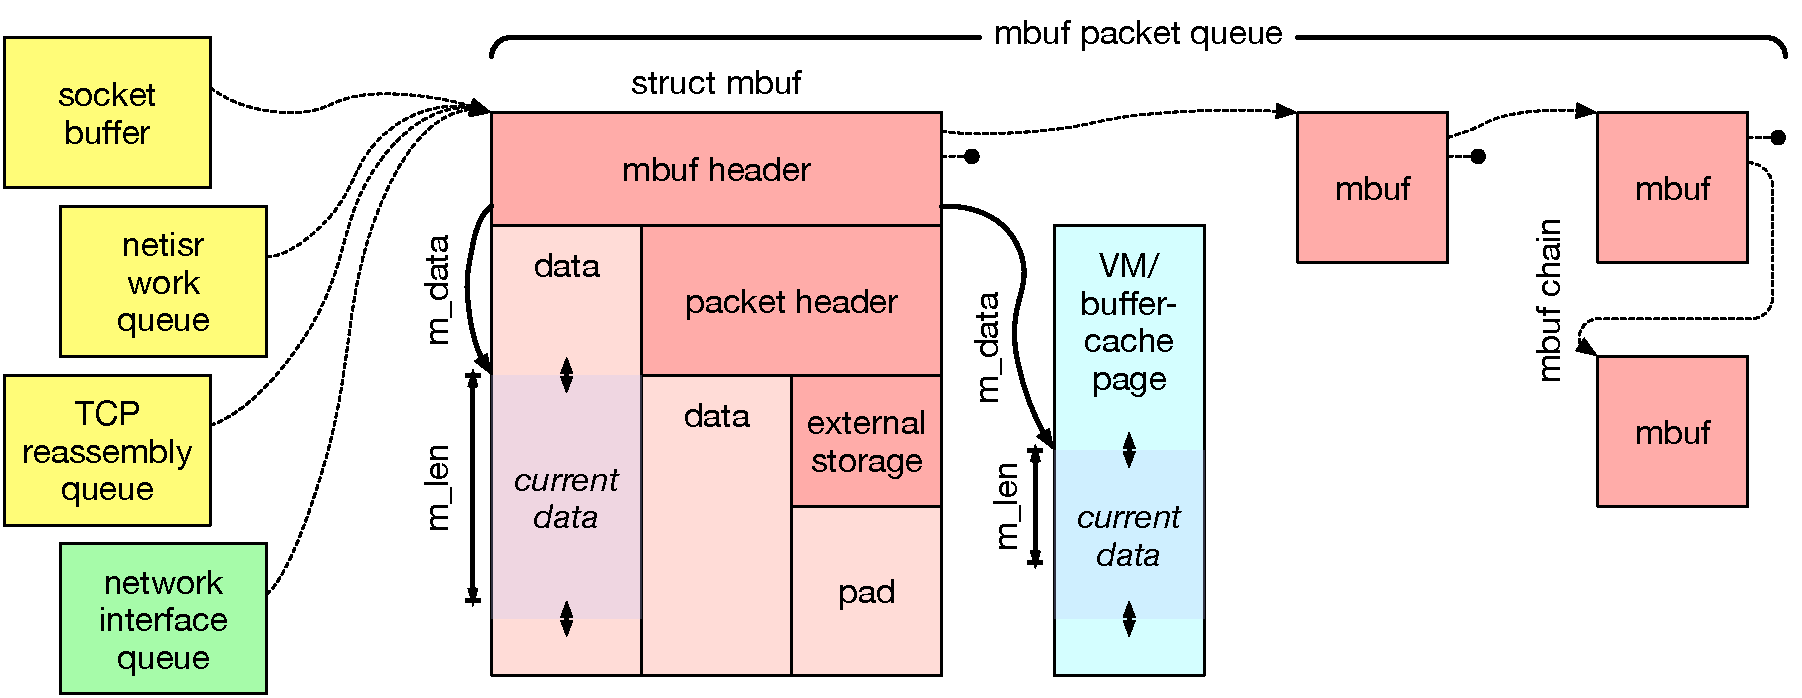
\includegraphics[width=\textwidth]{../../figures/network-mbufs.pdf}
  \end{center}

  \vspace{-0.45cm}
  \pause

  \begin{itemize}
    \item \texttt{mbuf} chains represent in-flight packets, streams, etc.

    \pause

    \begin{itemize}
      \item Ops: alloc, free, prepend, append, truncate, enqueue, dequeue
      \item Internal or external data buffer (e.g., VM page)
      \item Bi-modal packet-size distribution; e.g., TCP ACKs vs. data
    \end{itemize}

    \smallskip
    \pause

    \item Unit of \textbf{work allocation and distribution} throughout the
      stack
    \pause
    \item Similar structures in other OSes -- e.g., \texttt{skbuff} in Linux
    %\item Extraordinarily 1980s data structure -- and very hard to change!
  \end{itemize}
\end{frame}

\begin{frame}
  \frametitle{Local send/receive paths in the network stack}
  \begin{center}
    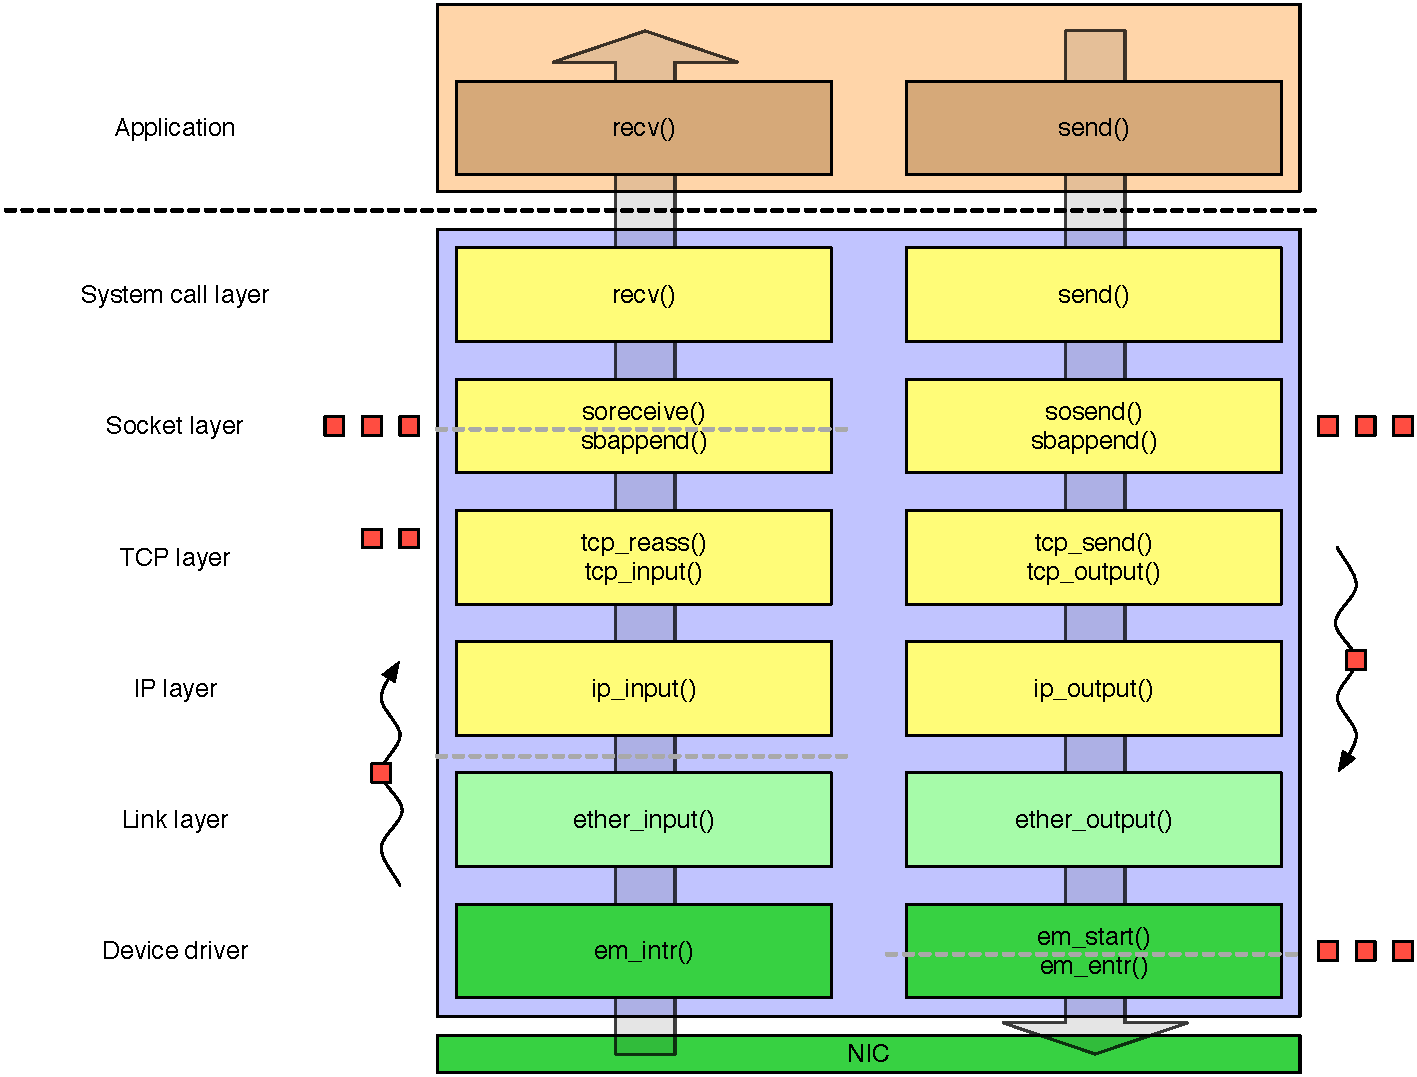
\includegraphics[scale=0.4]{../../figures/network-in-out.pdf}
  \end{center}
\end{frame}

\begin{frame}
  \frametitle{Forwarding path in the network stack}
  \begin{center}
    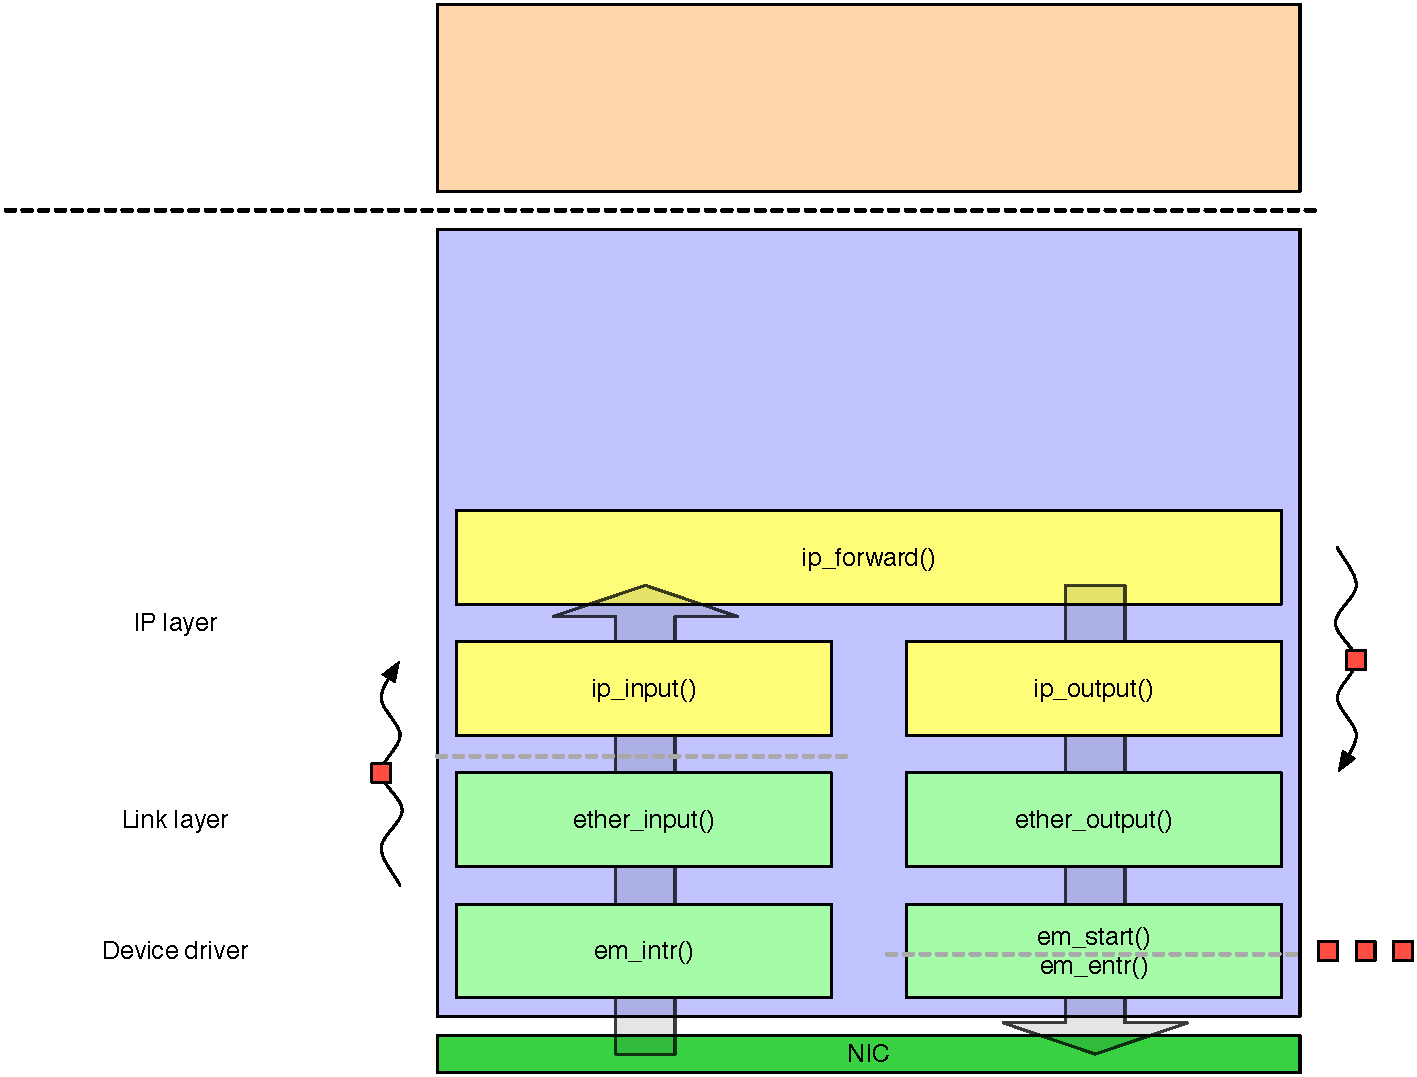
\includegraphics[scale=0.4]{../../figures/network-forward.pdf}
  \end{center}
\end{frame}

\begin{frame}
  \frametitle{Work dispatch: input path}

  \begin{center}
    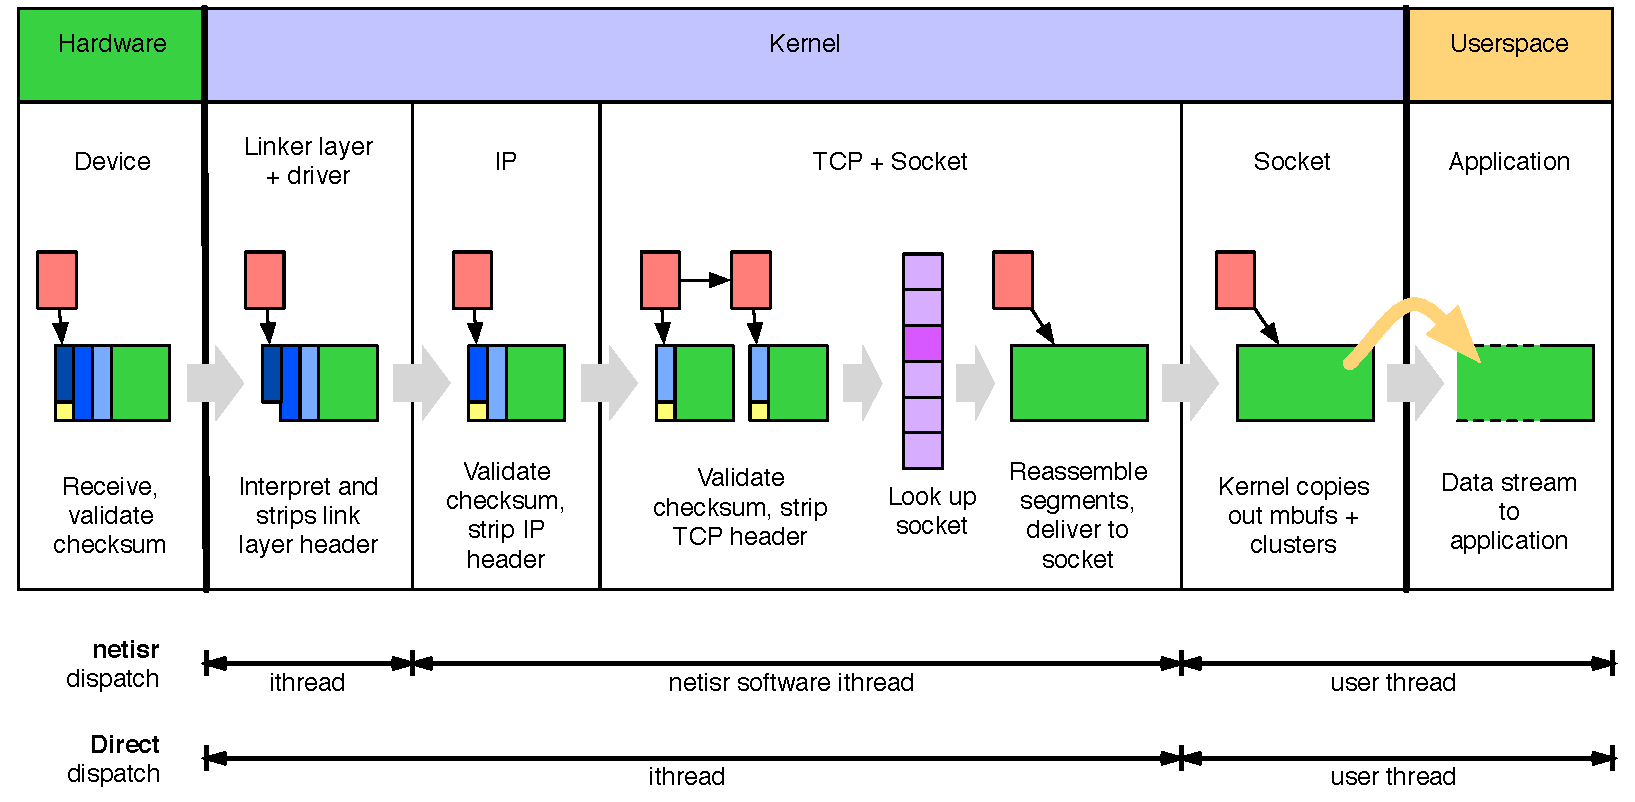
\includegraphics[width=0.9\textwidth]{../../figures/network-dispatch-input.pdf}
  \end{center}

  \begin{small}
  \begin{itemize}
    \pause
    \item Deferred dispatch - \textit{ithread} -> \textit{netisr thread} ->
      \textit{user thread}

    \pause

    \item Now: direct dispatch - \textit{ithread} -> \textit{user thread}
    \begin{itemize}
      \item Pros: reduced latency, better cache locality, drop overload early
      \item Cons: reduced parallelism and work placement opportunities
    \end{itemize}
  \end{itemize}
  \end{small}
\end{frame}

\begin{frame}
  \frametitle{Work dispatch: output path}

  \begin{center}
    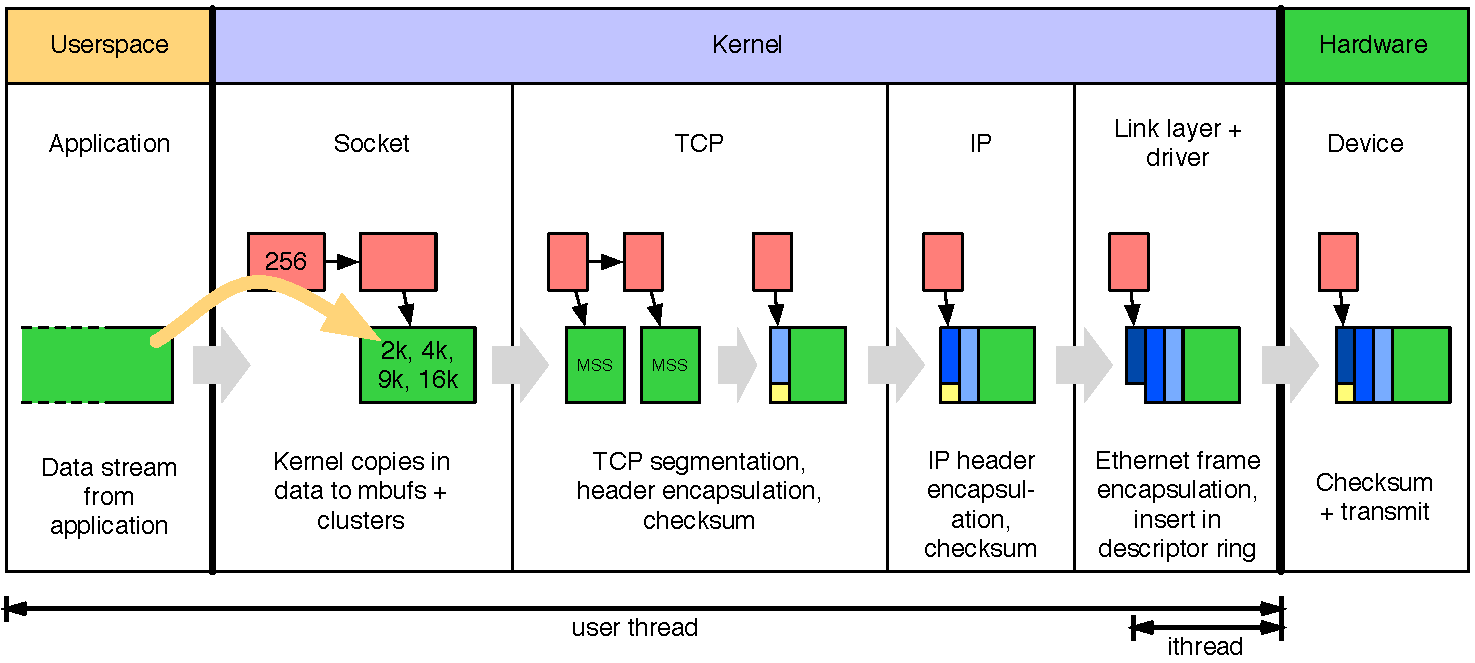
\includegraphics[width=0.9\textwidth]{../../figures/network-dispatch-output.pdf}
  \end{center}

  \pause

  \begin{itemize}
    \item Fewer deferred dispatch opportunities implemented

    \pause

    \item Gradual shift of work from software to hardware
    \begin{itemize}
      \item Checksum calculation, segmentation, ...
    \end{itemize}
  \end{itemize}

\end{frame}

\begin{frame}
  \frametitle{Work dispatch: TOE input path}

  \begin{center}
    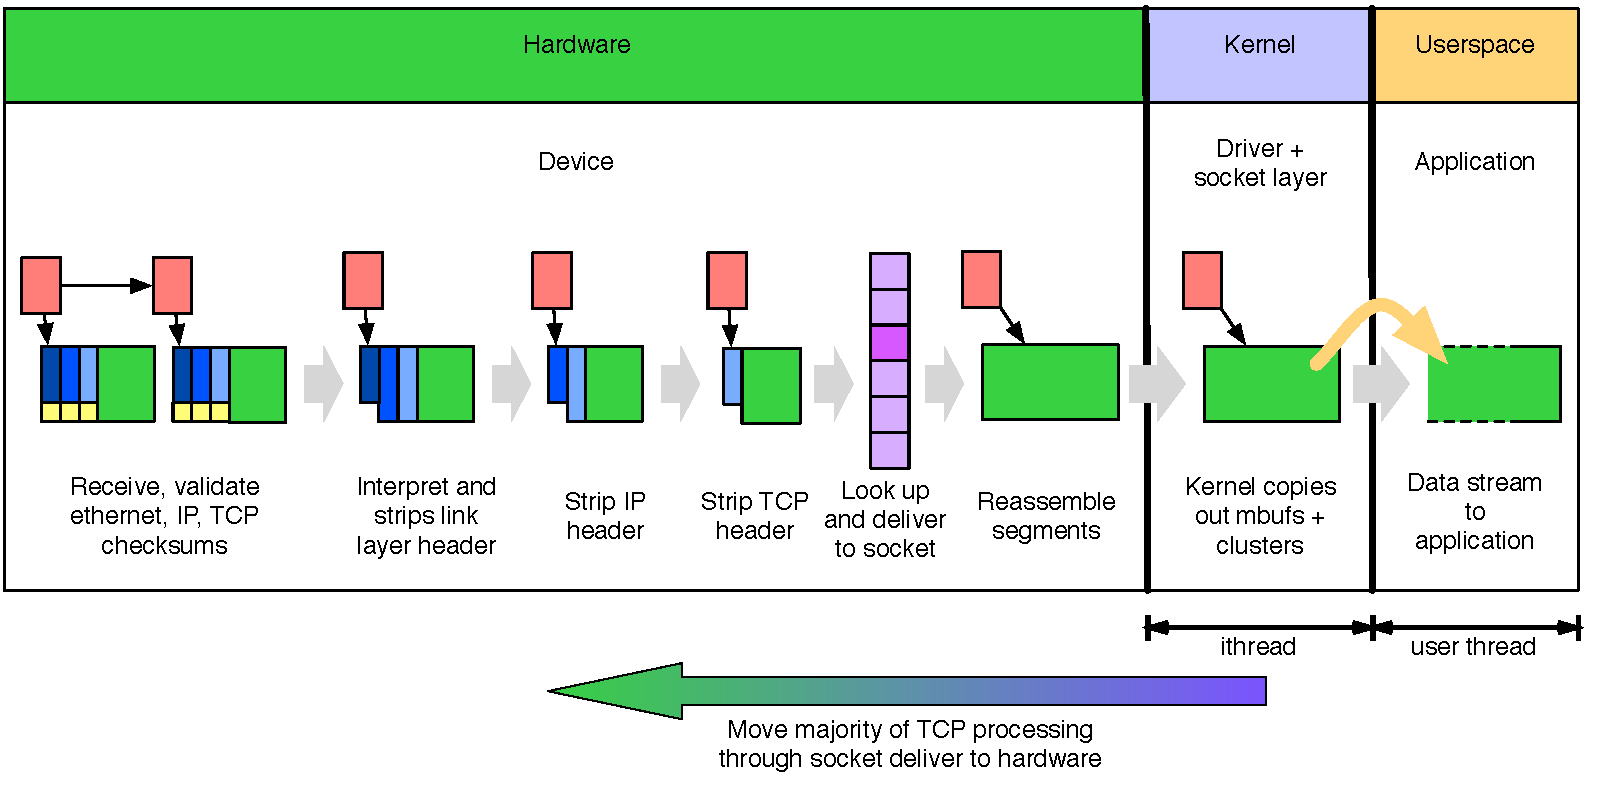
\includegraphics[width=0.9\textwidth]{../../figures/network-dispatch-toe.pdf}
  \end{center}

  \vspace{-0.5cm}
  \pause

  \begin{small}
  \begin{itemize}
    \item Full TCP offload
    \begin{itemize}
      \item Kernel provides socket buffers and resource allocation
      \item Remainder, including state, retransmits, reassembly, etc, in NIC
    \end{itemize}

    \smallskip
    \pause

    \item But: Two network stacks?  Less flexible/updateable structure?
    \item Better with an explicit HW/SW architecture -- e.g., Microsoft Chimney?
  \end{itemize}
  \end{small}
\end{frame}

%\begin{frame}
%  \frametitle{\texttt{sendfile}}
%
%  \begin{itemize}
%    \item XXX
%  \end{itemize}
%\end{frame}

%\begin{frame}
%  XXX: UNIX (or local) domain sockets \\
%  XXX: socket buffer to socket buffer
%\end{frame}
%
%\begin{frame}
%  XXX: Socket buffers and flow control
%\end{frame}
%
%\begin{frame}
%  XXX: Packetisation
%\end{frame}

%\begin{frame}
%  XXX: Concurrency and threading \\
%  XXX: Timers (RTT measurement, timeouts, rate control, ...)
%\end{frame}

%\begin{frame}
%  XXX: Ifnet -- the other end of the stack \\
%  XXX: Device drivers vs. the ifnet abstraction
%\end{frame}

%\begin{frame}
%  XXX: What a network device driver does
%\end{frame}

%\begin{frame}
%  XXX: Thinking about the link layer (ethernet .. 802.11)
%\end{frame}

%\begin{frame}
%  XXX: The input path
%\end{frame}
%
%\begin{frame}
%  XXX: The output path
%\end{frame}
%
%\begin{frame}
%  XXX: the netisr
%\end{frame}
%
%\begin{frame}
%  XXX: A bit of tracing
%\end{frame}

\section{Current research}

\begin{frame}
  \frametitle{netmap: a novel framework for fast packet I/O}

  Luigi Rizzo, USENIX ATC 2012 (best paper).

  \begin{columns}[T]
    \column{0.45\textwidth}

      \smallskip
      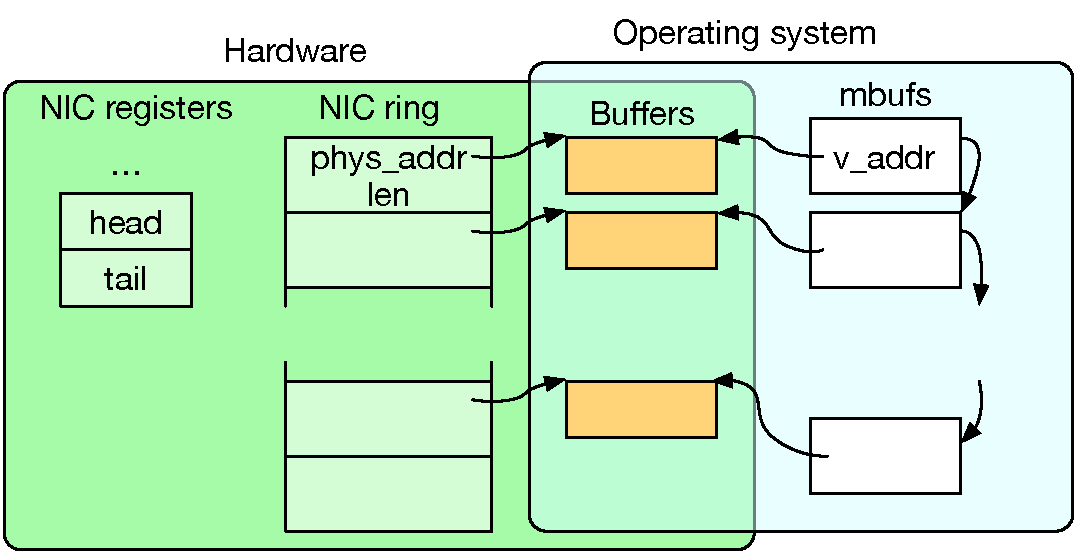
\includegraphics[width=1.1\textwidth]{../../figures/network-nic-stack.pdf}

      \bigskip
      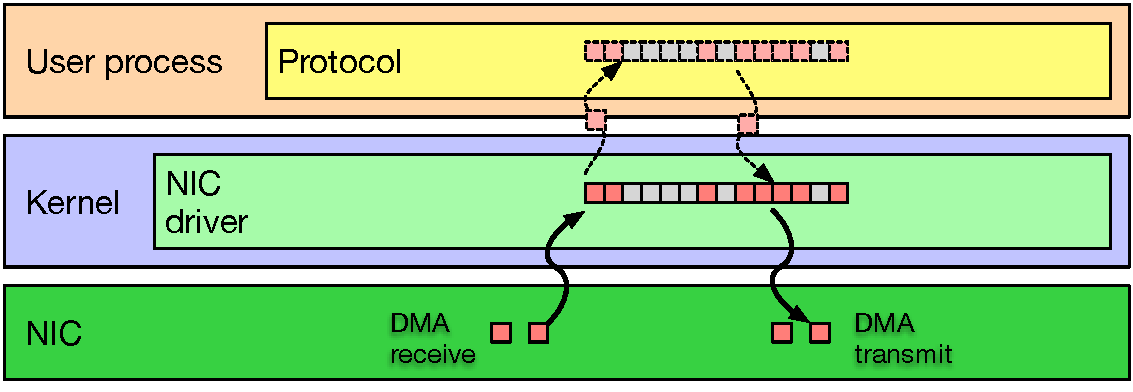
\includegraphics[width=1.1\textwidth]{../../figures/network-netmap-memory-flow.pdf}

    \column{0.45\textwidth}

    \pause

    \begin{itemize}
      \item Map NIC buffers directly into user process memory
      \item Zero copy to/from app.

      \medskip
      \pause

      \item System calls initiate DMA, block for NIC events
      \item Packets can be reinjected into normal stack
      \item Ships in FreeBSD, patch available for Linux

      \medskip
      \pause

      \item Userspace network stack can be \textbf{specialized} to task
	(e.g., packet forwarding)
    \end{itemize}
  \end{columns}
\end{frame}

\begin{frame}
  \frametitle{Network Stack Specialization for Performance}

  Ilias Marinos, Robert N.M. Watson, Mark Handley, SIGCCOMM 2014.

  \smallskip

  \begin{columns}[T]
    \column{0.45\textwidth}

    \smallskip
    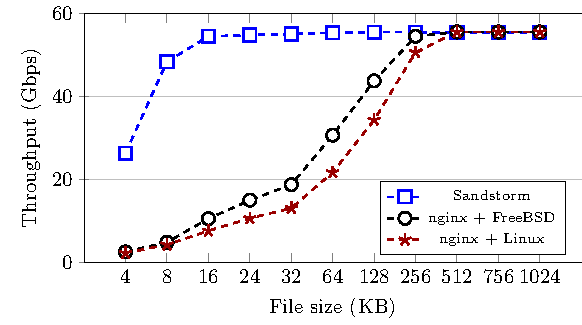
\includegraphics[scale=0.61]{../../figures/throughput_nginx_sandstorm_6nics_new.pdf} \\
    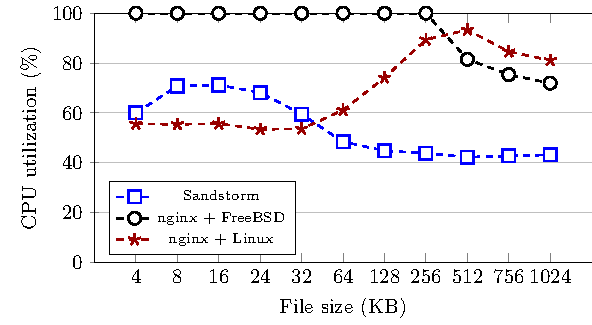
\includegraphics[scale=0.61]{../../figures/cpu_nginx_sandstorm_6nics_new.pdf}

    \column{0.45\textwidth}

    \pause

    \begin{itemize}
      \item 30 years since network-stack design developed

      \medskip
      \pause

      \item Massive changes in architecture, micro-architecture, memory,
	buses, NICs
      \begin{itemize}
	\item Optimising compilers
	% NB: first processor with cache in roughly 1984 -- after TCP and UDP!
	\item Cache-centered CPUs
	\item Multiprocessing, NUMA
	\item DMA, multiqueue
	\item 10 Gigabit/s Ethernet
      \end{itemize}

      \medskip
      \pause

      \item Revisit fundamentals through clean-slate stack
    \end{itemize}
  \end{columns}
\end{frame}

\section{Conclusion}

\begin{frame}[fragile]
  \frametitle{Next time: Socket buffers and TCP}

  \begin{columns}[T]
    \column{0.5\textwidth}

  \begin{Tiny}
    \begin{verbatim}
September 1981                             Transmission Control Protocol
                                                Functional Specification

                              +---------+ ---------\      active OPEN  
                              |  CLOSED |            \    -----------  
                              +---------+<---------\   \   create TCB  
                                |     ^              \   \  snd SYN    
                   passive OPEN |     |   CLOSE        \   \           
                   ------------ |     | ----------       \   \         
                    create TCB  |     | delete TCB         \   \       
                                V     |                      \   \     
                              +---------+            CLOSE    |    \   
                              |  LISTEN |          ---------- |     |  
                              +---------+          delete TCB |     |  
                   rcv SYN      |     |     SEND              |     |  
                  -----------   |     |    -------            |     V  
 +---------+      snd SYN,ACK  /       \   snd SYN          +---------+
 |         |<-----------------           ------------------>|         |
 |   SYN   |                    rcv SYN                     |   SYN   |
 |   RCVD  |<-----------------------------------------------|   SENT  |
 |         |                    snd ACK                     |         |
 |         |------------------           -------------------|         |
 +---------+   rcv ACK of SYN  \       /  rcv SYN,ACK       +---------+
   |           --------------   |     |   -----------                  
   |                  x         |     |     snd ACK                    
   |                            V     V                                
   |  CLOSE                   +---------+                              
   | -------                  |  ESTAB  |                              
   | snd FIN                  +---------+                              
   |                   CLOSE    |     |    rcv FIN                     
   V                  -------   |     |    -------                     
 +---------+          snd FIN  /       \   snd ACK          +---------+
 |  FIN    |<-----------------           ------------------>|  CLOSE  |
 | WAIT-1  |------------------                              |   WAIT  |
 +---------+          rcv FIN  \                            +---------+
   | rcv ACK of FIN   -------   |                            CLOSE  |  
   | --------------   snd ACK   |                           ------- |  
   V        x                   V                           snd FIN V  
 +---------+                  +---------+                   +---------+
 |FINWAIT-2|                  | CLOSING |                   | LAST-ACK|
 +---------+                  +---------+                   +---------+
   |                rcv ACK of FIN |                 rcv ACK of FIN |  
   |  rcv FIN       -------------- |    Timeout=2MSL -------------- |  
   |  -------              x       V    ------------        x       V  
    \ snd ACK                 +---------+delete TCB         +---------+
     ------------------------>|TIME WAIT|------------------>| CLOSED  |
                              +---------+                   +---------+

                      TCP Connection State Diagram
                               Figure 6.
\end{verbatim}
  \end{Tiny}

    \column{0.4\textwidth}

    \pause

    \begin{itemize}
      \item McKusick, et al: Chapter 14 (\textit{Transport-Layer Protocols})

      \medskip
      \pause

      \item Transmission Control Protocol (TCP)
      \item TCP implementation
      \begin{itemize}
	\item Buffers and input processing
	\item Parallelism and performance
	\item DoS resistance
      \end{itemize}

      \medskip
      \pause

      \item The final two labs
    \end{itemize}
  \end{columns}

\end{frame}

\end{document}
